\documentclass{article}

\usepackage[export]{adjustbox}
\usepackage{listings}
\usepackage{subcaption}
\usepackage{wrapfig}
\usepackage[dvipsnames]{xcolor}
\usepackage{alloy-style}
\usepackage{float}
\usepackage{graphicx}
\usepackage[utf8]{inputenc}
\usepackage[a4paper, top=4cm, bottom=4cm, left=4cm, right=4cm]{geometry}

\title{
    \textbf{\textit{SafeStreets}} \\
    \textbf{RASD document}}

\date{Academic year: 2019 - 2020}
\author{
    Dario Miceli Pranio \\
    Pierriccardo Olivieri
}

\begin{document}
\pagenumbering{gobble}

\maketitle

%%%%%%%%%% LOGO POLIMI %%%%%%%%%%
\begin{figure}[h!]
    \centering
    
\includegraphics[scale=0.5]{img/logo.png}
\end{figure}

\newpage
\pagenumbering{arabic}
\tableofcontents

\newpage
%%%%%%%%%% CHAPTER 1 %%%%%%%%%%
\section{Introduction}
This is the RASD document for \textit{SafeStreets}, that provides a general view about key aspects of the project. 
The purpose of this document is to formalize a description of the \textit{System's} requirements both functional and non-functional. 
In the following pages will be covered goals of the application with respect to phenomena. This document is addressed to 
developers as a guideline to implement the requirements that follows and as an overview for stakeholders.

\subsection{Purpose}
\textit{SafeStreets} is a service that aims to provide \textit{Users} with the possibility to notify \textit{Authorities} when traffic 
violations occur, and in particular parking violations. The application's goal is achieved by allowing \textit{Users} 
to share photo, position, date, time and type of violation and by enabling \textit{Authorities} to request them.
\\
\\
\textit{SafeStreets} requires the \textit{Users} to create an account to access its services, the functionalities unlocked after 
registration depend on the type of account created.
\\
If a \textit{User} creates an account as \textit{Citizen}, he/she must provide name, surname and a fiscal code in order to prove 
that he/she is a real person. Furthermore, he must provide an email with which he will be uniquely identified 
and a password. Once the account has been activated, \textit{User} can finally start to report parking violations and can also see 
statistics of the streets or the areas with the highest frequency of violations.
\\
\\
On the other hand, an officer will create an account as \textit{Authority} and he will need to provide his name, surname, 
work's Matricola, a password and as for \textit{Citizen}, will be uniquely identified by an email. Once the Matricola 
has been verified and the account has been activated, the officer can retrieve the potential parking violations 
sent by \textit{Citizen} that have not been taken into account yet by other officers, analyze them and, if it is the 
right case, generates traffic tickets. \textit{Authorities}, can see the same statistics of the \textit{Citizen} and can also see
statistics about vehicles' license plate that commit the most violations.
\\
\\
From this brief description of the functionalities we may extract the following goals for \textit{SafeStreets}:
\begin{itemize}
    \item \textbf{[G1]}: Allow \textit{Guest} to be registered as a \textit{Citizen} or as \textit{Authority};
    \item \textbf{[G2]}: Allow \textit{Citizens} to report parking violations;
    \item \textbf{[G3]}: \textit{Citizen} has to be able to input information about the violation that he has reported;
    \item \textbf{[G4]}: Must provide a visualization of the areas with high frequency of violations to \textit{Users};
    \item \textbf{[G5]}: Must provide a visualization of vehicles that commit the most violations to \textit{Authorities}; 

\end{itemize}
\textit{SafeStreets} offers also some advanced functions in addition to the basic version.
\begin{itemize}
    \item \textbf{[G6]}: Must ensure the chain of custody of the information sent by \textit{Citizens};
    \item \textbf{[G7]}: \textit{Authorities} can retrieve traffic violations' in order to generate traffic tickets;
    \item \textbf{[G8]}: \textit{System} must build statistics with the informations about issued tickets;
\end{itemize}

\subsection{Scope}
Here we will describe all the relevant phenomena that may occur. 

\subsubsection{World Phenomena}
Those are the events that may occur in the real word and are not affected by the Machine.
\\We identify:
\begin{itemize}
    \item \textit{Citizen} sees a parking violation and wants to report it;
    \item \textit{Users} want to know about some violations that have been occurred;
    \item A \textit{parking violation} occurs; 
\end{itemize} 

\subsubsection{Shared Phenomena}
Shared phenomena are the events based on the link beetween World Phenomena and Machine Phenomena.
We can distinguish them in two types:
\\
Controlled by the world observed by the machine:
\begin{itemize}
    \item A \textit{Citizen} reports a violation;
    \item \textit{Users} can enter data for registration/login;
    \item \textit{Users} can request data;
\end{itemize}
Controlled by the machine observed by the world:
\begin{itemize}
    \item Track position of the violation;
    \item Mark areas with an high rate of violations;
    \item \textit{System} can fullfill data requests;
\end{itemize}

\subsubsection{Machine Phenomena}
The Machine Phenomena are the events that occur inside the machine and are not affected by the real world.
\\We identify:
\begin{itemize}
    \item Storing permanently collected data;
    \item Encryption of sensitive data;
    \item Retrieving data for a request; 
\end{itemize} 

\subsection{Definitions, acronyms, abbreviations}

\subsubsection{Definitions}
\begin{itemize}
    \item \textit{Users}: can be either \textit{Citizen} or \textit{Authority}
    \item \textit{traffic violation}: generic violation that can occur in a street
    \item \textit{parking violation}: a violation caused by a bad parking
    \item \textit{violation}: general violation, identity both traffic or parking violation
    \item \textit{unsafe areas}: areas with an high rate of violations
\end{itemize}

\subsubsection{Acronyms}
Table with all acronyms used in document.
\begin{center}
\begin{tabular}{ | l | l |}
    \hline
    ACRONYM & COMPLETE NAME \\
    \hline
    RASD & Requirements Analysis and Specification Document \\
    \hline
    GPS & Global Positioning Systems \\
    \hline
    S2B & Software To Be \\
    \hline
    GDPR & General Data Protection Regulation \\
    \hline 
    FC & Fiscal Code \\
    \hline
    UC & Use Case \\
    \hline
\end{tabular}
\end{center}

\subsubsection{Abbreviations}
\begin{itemize}
    \item \textbf{Gn}: n-th Goal
    \item \textbf{Rn}: n-th Requirement 
    \item \textbf{Dn}: n-th Domain Assumption
    \item \textbf{Cn}: n-th Constraint 
    \item \textbf{UCn}: n-th Use Case
\end{itemize}

\subsection{Revision History}

\subsection{Reference documents}
\begin{itemize}
    \item ISO/IEC/IEEE 29148: https://www.iso.org/standard/45171.html
    \item Specification Document: "SafeStreets Mandatory Project Assignement"
    \item Diagrams: https://www.draw.io/
    \item Mockups: https://www.figma.com/
    \item Alloy Official Documentation: http://alloy.lcs.mit.edu/alloy/documentation.html
    \item Alloy code highlithing for Latex: https://github.com/Angtrim/alloy-latex-highlighting
\end{itemize}

\subsection{Document Structure}
\begin{itemize}
    \item \textbf{Chapter 2}: Presents an overall description of the \textit{System} explaining in more datailed 
    way Phenomena described in chapter 1. Provides some diagrams usefull to understand key aspects and 
    general behavior of the \textit{System} and possible type of \textit{Users} with respective functions that they are allowed to do. 
    This chapter is also focused on defining functional requirements such
    as constraints, domain assumption and dependencies that will be covered later.    
    \item \textbf{Chapter 3}: This chapter is intended for developers, dives deeper on the aspects of chapter 2 using 
    use cases and sequence diagrams in order to clarify process and interaction between \textit{Users} and \textit{System}. 
    Describe the interfaces for the application, focusing on \textit{System}'s design constraints and software \textit{System} attributes.  
    \item \textbf{Chapter 4}: Uses Alloy to generate a Formal Model for the application.
\end{itemize}
%%%%%%%%%% !CHAPTER 1 %%%%%%%%%%

\clearpage

%%%%%%%%%% CHAPTER 2 %%%%%%%%%%
\section{Overall Description}

\subsection{Product perspective}
This section aims to explain in more detail the World, Machine and Shared Phenomena described in the 
previous Chapter. 

\subsubsection{World Phenomena}
\begin{itemize}
    \item \textbf{Citizen sees a parking violation and wants to report it}:
    While the \textit{Citizen} is quietly walking, he sees a parking violations like a double parking or a car
    parked in the middle of bike lane and wants to report it.
    \item \textbf{Users want to know abount some violations that have been occurred}:
    An \textit{User} has the needs to check some statistics about parking violations on a certain area
    for some purpose.
    \item \textbf{A parking violation occurs}:
    Someone in the city decides to not follow parking rules and doesn't park his car in a proper way.
\end{itemize}

\subsubsection{Machine Phenomena}
\begin{itemize}
    \item \textbf{Storing permanently collected data}:
    The \textit{System} needs to store, in a secure way, all the data submitted.
    In order to achieve this purpose and guarantee the best service
    the \textit{System} needs to use a DBMS.
    \item \textbf{Encryption of sensitive data}:
    Personal \textit{User's} data and all the data relative to the violations
    that can only be seen by \textit{Authorities} need to be encrypted in order
    to proctect it from non-allowed third parties. 
    \item \textbf{Retrieving data for a request}:
    \textit{System} has to fullfill the data request from the \textit{Users}. Data 
    requests can be of two types, a \textit{Citizen} request to see
    statistics of a certain city area or data request by \textit{Authorities}
    who want to receive the violation reports collected by \textit{SafeStreets} or 
    statistics about unsafe city areas and vehicles.
\end{itemize}

\subsubsection{Shared Phenomena}
Controlled by the World observed by the Machine
\begin{itemize}
    \item \textbf{A Citizen reports a violation}:
    Situation in which a \textit{Citizen} spots a generic violation and wants
    to report it through the application. Using \textit{SafeStreets} he
    can take the photo of the violation.
    \item \textbf{User can enter data for registration/login}:
    A \textit{User} decide to use the application and provides his personal data
    in order to register if it's the first time he use the app, or to
    identify himself.
    \item \textbf{Users can request data}:
    In this phenomena we make a distinction between \textit{Citizen} and \textit{Authorities}.
    A \textit{Citizen} may want to see violation statistics of a certain area, \textit{Authorities} can request
    violation statistics and most egregious offender's vehicles statistics.
\end{itemize}

Controlled by the Machine observed by the World
\begin{itemize}
    \item \textbf{Track position of the violation}:
    The \textit{System} can retrieve the position where the violation occurred by fetching it from GPS service.
    \item \textbf{Mark areas with an high rate of violations}:
    Once some violations have been occured, the \textit{System} mines the information that it has in 
    order to highlight the areas with the highest frequency of violations.
    \item\textbf{System can fullfill data requests}:
    After processing a request, the \textit{System} will show to the \textit{User} the result of the 
    DBMS query in a proper way.
\end{itemize}

\subsubsection{Class Diagram} 

\begin{figure}[h!]
    \centering
    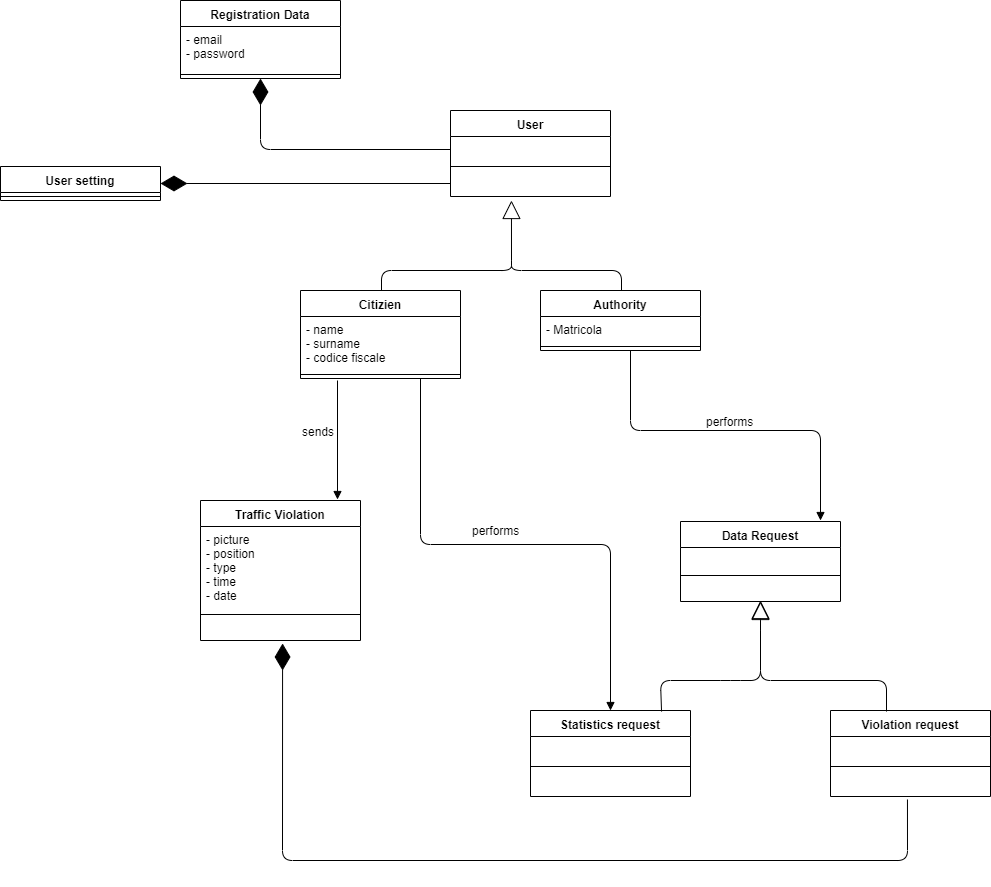
\includegraphics[scale=0.3]{img/class_diagram.png}
    \caption{\textit{SafeStreets'} Class diagram}
\end{figure}
\clearpage
\subsubsection{State Charts} 

\begin{figure}[h!]
    \centering
    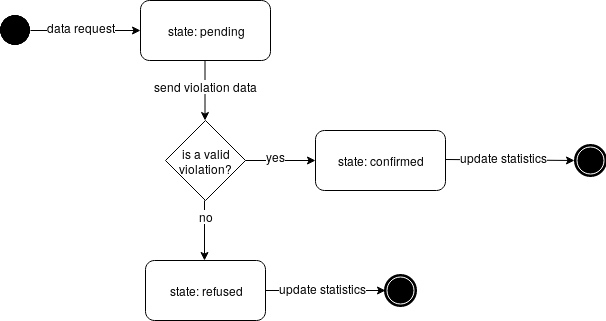
\includegraphics[scale=0.5]{img/state_charts/authority_request.png}
    \caption{\textit{Authority} requests for violations state chart}
\end{figure}

\begin{figure}[h!]
    \centering
    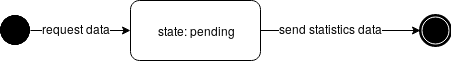
\includegraphics[scale=0.5]{img/state_charts/citizen_request.png}
    \caption{\textit{Users} request statistics state chart}
\end{figure}

\subsection{Product functions}
In this section are explained the functions associated to \textit{User}.
\begin{itemize}
    \item \textbf{Citizen functions}:
    \\
    \\
    \textbf{Report a violation}
    \\When a \textit{Citizen} sees a parking violation, he takes a picture of the vehicle paying attenction to focus on the 
    license plate, inputs the type of the violation and sends it. The \textit{System} will provide to add the position retrieving 
    from GPS, to add the right time and date and to add the license plate obtained through the algorithm and confirmed by
    the \textit{Citizen}. 
    \\
    \\
    \textbf{Retrieve statistics about unsafe areas}
    \\\textit{Safestreets} enables \textit{Citizen} to visualize statistics about \textit{unsafe areas}. \textit{SafeStreets} 
    mines the informations it has and let the \textit{Citizen} retrieves the result through a clear interface containing 
    significant plots, tables and charts. 

    \item \textbf{Authority functions}:
    \\
    \\
    \textbf{Retrieve statistics about unsafe areas}
    \\\textit{Safestreets} enables \textit{Authority} to visualize statistics about unsafe areas. \textit{SafeStreets} mines the 
    informations it has and let the \textit{Authority} retrieves the result through a clear interface containing significant plots, 
    tables and charts.
    \\
    \\
    \textbf{Retrieve statistics about vehicles}
    \\\textit{Safestreets} enables \textit{Authority} to visualize statistics about vehicles. \textit{SafeStreets} mines the 
    informations it has and let the \textit{Authority} retrieves the result through a clear interface containing 
    significant plots, tables and charts about most egregious offenders.
    \\
    \\
    \textbf{Request violations data for traffic tickets}
    \\\textit{SafeStreets} enables \textit{Authority} to retrieve all the parking violations sent by \textit{Citizens}. For each 
    parking violation \textit{Authority} can accepts it or declines it. In the first case he can generates traffic ticket, 
    in the second case he discards the informations about the parking violations. In both cases \textit{SafeStreets} records 
    response in order to build statistics.

\end{itemize}

\subsection{User characteristics}
Below we describe the convention used to identify the \textit{Users} of the application and the function that those 
\textit{Users} are allow to perform.
\begin{itemize}
    \item \textbf{Guest}: A \textit{User} that have donwloaded the application but is not 
    registered yet. This type of \textit{User} is not allowed to access 
    the application functionalities.
    \item \textbf{Citizen}: is a generic \textit{User} app not related to \textit{Authorities}, a 
    common \textit{Citizen} that wants to use the application. After the registration process, he can 
    log in the application and use the functionalities such as report a violation or request 
    informations about the statistics of a certain area.
    \item \textbf{Authority}: This \textit{User} is associated to the local municipal
    police district, any traffic warden, once registered with 
    is matricola number and logged in have full access to statistics, both violations and vehicles, and 
    can request all the violations reported from \textit{Citizens} in order to generate traffic tickets. 
    \item \textbf{User}: can be both a \textit{Citizen} or \textit{Authority} type, in this document
    this name is used when it's not necessary make a distinction 
    between the two.
\end{itemize}

\subsection{Assumption and Dependencies Constraints}
\subsubsection{Domain Assumption}
The following list present all the domain assumption made.
\begin{itemize}
    \item \textbf{[D1]}: \textit{Users} can't make more than one account.
    \item \textbf{[D2]}: The personal informations provided by \textit{User} are valid and belongs to the him.
    \item \textbf{[D3]}: Position data as an accuracy of 10 meters.
    \item \textbf{[D4]}: The \textit{System} can access internet whenewer needs it.
    \item \textbf{[D5]}: Permission to access GPS data is always allowed.
    \item \textbf{[D6]}: Permission to take a photo is always allowed. 
\end{itemize}

\subsubsection{Dependencies}
This list below represent all the dependencies that S2B need in order to work properly.
\begin{itemize}
    \item Smartphone needs an internet connection.
    \item Smartphone needs a Photocamera.
    \item Smartphone needs a GPS system.
    \item \textit{SafeStreets} needs a trusted external storage for violations data and personal data.
\end{itemize}

\subsubsection{Constraints}
\begin{itemize}
    \item The S2B must guarantee the European data protection GDPR for \textit{User's} sensitive data.
    \item The S2B will be used only in Italy due to personal data type like (fiscal code and police matricola).
    \item The S2B will be developed as a smartphone application.
    \item The \textit{Citizen} can only take photos from the application. 
\end{itemize}
%%%%%%%%%% !CHAPTER 2 %%%%%%%%%%

\clearpage
%%%%%%%%%% CHAPTER 3 %%%%%%%%%%
\section{Specific Requirements}

\subsection{External Interface Requirements}
\subsubsection{User Interfaces}

\paragraph{Login or register page}
This is the first page that \textit{Users} see after downloading and installing \textit{SafeStreets} 
application. Both \textit{Authorities} and \textit{Citizens} can log in from this page without 
distinction because they have to provide only email \& password. If \textit{User} hasn't been registered
yet in \textit{SafeStreets} can go to regisiter page by clicking on register button and the \textit{System} will
show the default register for \textit{Citizen}.
\\
\\
\\
\\
\begin{figure}[H]
    \centering
    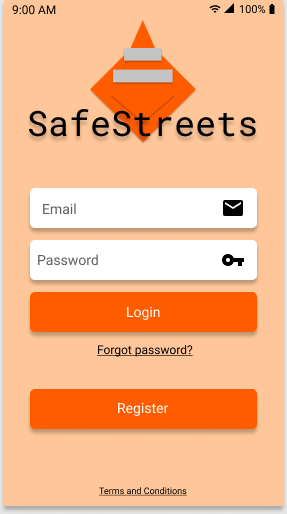
\includegraphics[scale=0.5]{img/mockups/login.png}
    \caption{Login or Register page}
\end{figure}

\clearpage

\paragraph{Registration page}
Registration pages ask \textit{Guests} to input name, surname, email and a password. If the \textit{Guest} is a \textit{Citizen}
he must also input his Fiscal Code otherwise if he is an \textit{Authority} he must input his Matricola. The default page that the 
\textit{System} shows when the register button is clicked is the \textit{Citizen} registration page. If the \textit{Guest} wants
to register him as \textit{Authority} he must click the "Register as \textit{Authority}" button. From this page it is possible
to return in the \textit{Citizen} registration page by clicking the "Register as \textit{Citizen}" button.   
\\
\\
\\
\\
\begin{figure}[H]
    \begin{subfigure}{0.5\textwidth}
        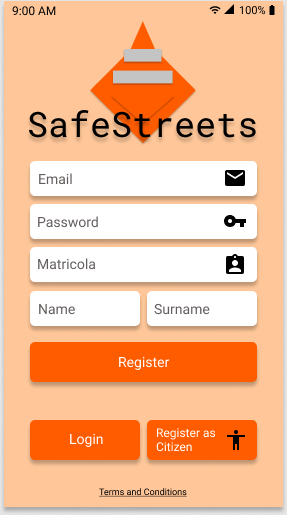
\includegraphics[width=0.9\linewidth]{img/mockups/register_authority.png} 
        \caption{Register for \textit{Authorities}}
        \label{fig:subim1}
    \end{subfigure}
    \begin{subfigure}{0.5\textwidth}
        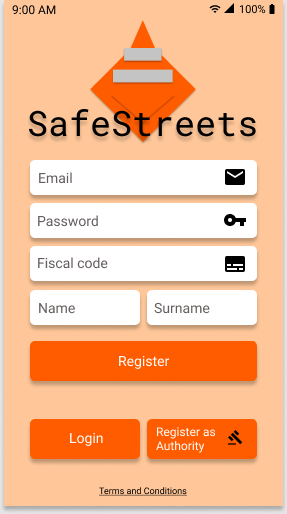
\includegraphics[width=0.9\linewidth]{img/mockups/register_citizen.png}
        \caption{Register for \textit{Citizens}}
        \label{fig:subim2}
    \end{subfigure}
    \caption{Registration pages}
    \label{fig:image2}
\end{figure}

\clearpage

\paragraph{Home pages}
\begin{itemize}
    \item \textbf{Citizen}: Home page shows a bar at the top of screen with some data such as name, surname, FC and 
    the number of violations reported. In the center of screen \textit{System} shows the open photocamera ready to take
    a picture by clicking the report button. It is possible to take a picture only if a license plate is framed with the 
    photocamera. Once the report button is clicked, a picture is taken and the \textit{Citizen} is redirected to the 
    \textit{Citizen} report info page. The two button at the bottom allow \textit{Citizen} to access statistics and 
    account's settings.

    \item \textbf{Authority}: Home page shows a bar at the top of screen with some data such as name, surname, Matricola,  
    the number of violations checked and the number of violation confirmed. In the center of screen there are 3 buttons:
    Retrieve Violation, Statistics, Vehicles statistics. The first one allows \textit{Authority} to access \textit{Authority} 
    report info page, the second one allows to access violation statistics and the last one allows to access vehicles 
    statistics. It is also present the settings button to access account's settings.  

\end{itemize}

\begin{figure}[H]
    \begin{subfigure}{0.5\textwidth}
        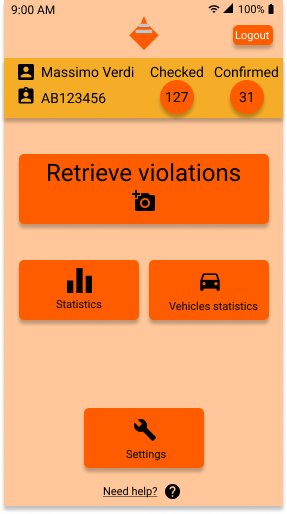
\includegraphics[width=0.9\linewidth]{img/mockups/home_authority.png} 
        \caption{Home page for \textit{Authorities}}
        \label{fig:subim1}
    \end{subfigure}
    \begin{subfigure}{0.5\textwidth}
        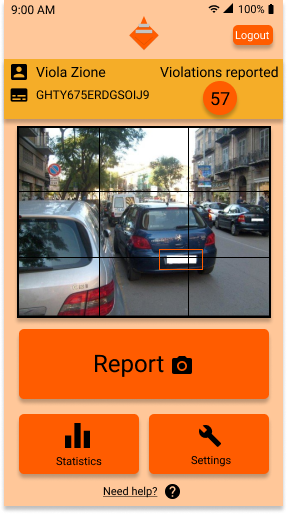
\includegraphics[width=0.9\linewidth]{img/mockups/home_citizen.png}
        \caption{Home page for \textit{Citizens}}
        \label{fig:subim2}
    \end{subfigure}
    \caption{Home pages}
    \label{fig:image2}
\end{figure}

\clearpage

\paragraph{Settings}
This two pages below represents the settings page in which the \textit{Citizen} and \textit{Authority} can change their 
personal data or visualize it. Only some informations can be modified, those who can't be modified are showed with 
grey color.
\\
\\
\\
\\
\begin{figure}[H]
    \begin{subfigure}{0.5\textwidth}
        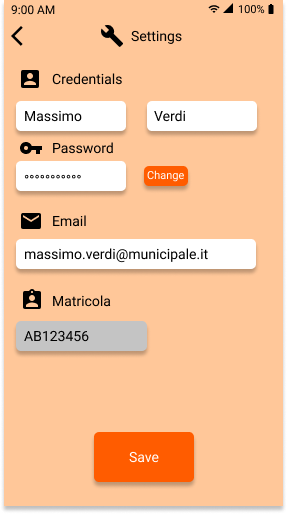
\includegraphics[width=0.9\linewidth]{img/mockups/settings_authority.png} 
        \caption{Settings for \textit{Authorities}}
        \label{fig:subim1}
    \end{subfigure}
    \begin{subfigure}{0.5\textwidth}
        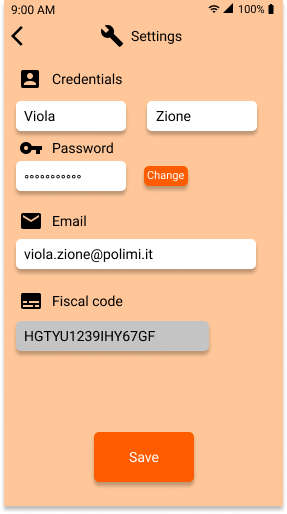
\includegraphics[width=0.9\linewidth]{img/mockups/settings_citizen.png}
        \caption{Settings for \textit{Citizens}}
        \label{fig:subim2}
    \end{subfigure}
    \caption{Settings Pages}
    \label{fig:image2}
\end{figure}

\clearpage

\paragraph{Statistics for Citizens}
In the page below we can see usefull statistics for \textit{Citizen}, there are 3 graphs that summarize all the interesting
informations. The first one shows the violations during a specific year, that can be changed in the filters below. 
The button 'type' can filter the violation's type to show only the type of interest, like 'double-parked' for instance. 
Those statistics are dislpayed with the violations number per month in the position selected. Below the map displays
a more generic view of the violations in a city by highlithing the zone with a color graduation that represent the most
dangerous zone. The more darker the more violations occur in that area, by changing the position in the map by clicking 
in a certain point the graph above will update the statistics for that area.  In the last gaph there is a perspective of 
the violations reported by \textit{Citizen} during a certain year that can be changed.
\\
\\
\\
\\
\begin{figure}[H]
    \centering
    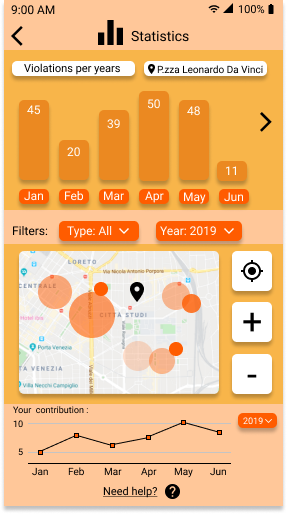
\includegraphics[scale=0.5]{img/mockups/statistics_citizen.png}
    \caption{Statistics \textit{Citizen}}
\end{figure}

\clearpage

\paragraph{Statistics for Authorities}
\begin{itemize}
    \item \textbf{Violations statistics}: The first two graph have the same function and are equale as the 
    two for \textit{Citizen}. The violations reported graph isn't present because \textit{Authority} can't 
    report a violation. In the bottom page there is a button for receive violation's statistics via mail.
    \item \textbf{Vehicles statistics}: In that page, that can only be seen by \textit{Authority} are showed 
    the statistics of the most egregious offender's vehicles. In the first part is possible to search for a 
    specific license plate, and if the vehicle related has commited some violations the stats will be displayed 
    below, divided per months and visualized by year, that can be changed.  Below are listed the license plate 
    of the most egregious offenders in a certain area selected at the top with the two buttons on the 
    right \textit{Authorities} can receive those data via specified mail. By clicking on a license plate 
    the bottom graph will be updated with the data relative to that, divided per month and visualized by year, 
    that can be changed with the button on the right.
\end{itemize}

\begin{figure}[H]
    \begin{subfigure}{0.5\textwidth}
        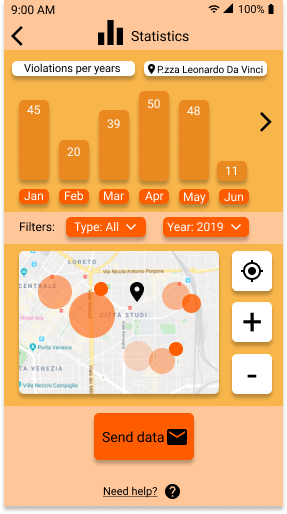
\includegraphics[width=0.9\linewidth]{img/mockups/statistics_authority_violations.png} 
        \caption{Violations Statistics}
        \label{fig:subim1}
    \end{subfigure}
    \begin{subfigure}{0.5\textwidth}
        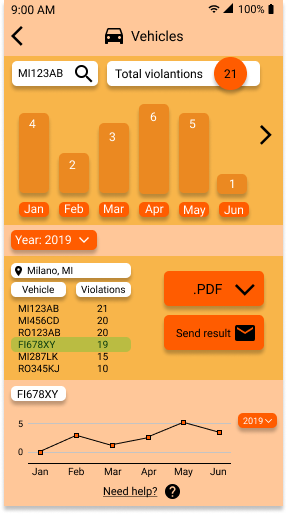
\includegraphics[width=0.9\linewidth]{img/mockups/statistics_authority_vehicles.png}
        \caption{Vehicle Statistics}
        \label{fig:subim2}
    \end{subfigure}
    \caption{Statistics for \textit{Authorities}}
    \label{fig:image2}
\end{figure}

\clearpage

\paragraph{Violation's report Citizen}
Below we can see the page that is displayed when a \textit{Citizen} clicks on the report button taking a photo of a
violation. In this page is showed the photo taken and some metadata retrivied automatically by the \textit{System} like
date, time, position and the license plate that is read by the algorithm. \textit{Citizen} can change the license plate
if the algorithm doesn't read it properly he can also choose the type of violation. The confirm button, if no error
occurs, will send the data collected to the \textit{System}.
\\
\\
\\
\\
\begin{figure}[H]
    \centering
    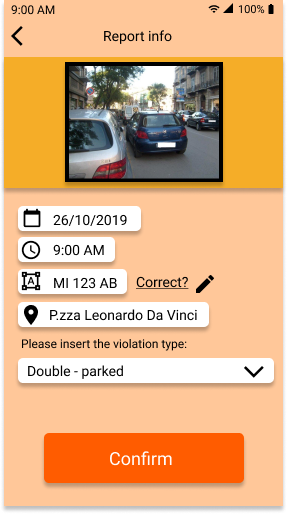
\includegraphics[scale=0.5]{img/mockups/page_citizen.png}
    \caption{Page \textit{Citizen}}
\end{figure}

\clearpage

\paragraph{Violation's check page for Authority}
In this page showed below the \textit{Authority} can confirm the violations reported by \textit{Citizen} and they can
generate traffic tickets from the data. In the page are showed the photo and the data necessary for the traffic ticket.
The \textit{Authority} can also receive this data by clicking on the button in the bottom.
\\
\\
\\
\\ 
\begin{figure}[H]
    \centering
    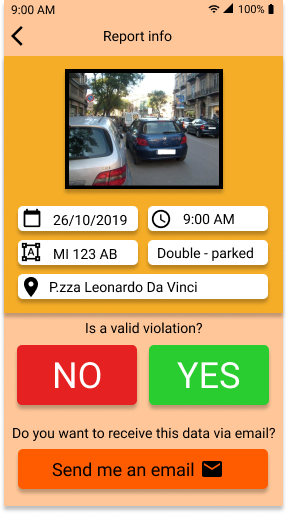
\includegraphics[scale=0.5]{img/mockups/page_authority.png}
    \caption{Page \textit{Authority}}
\end{figure}

\subsubsection{Hardware Interfaces}
The \textit{System} does not offer any Hardware Interfaces
\subsubsection{Software Interfaces}
As mobile applications, the main software interfaces are:
\begin{itemize}
    \item iOs
    \item Android
\end{itemize}
\subsubsection{Communication Interfaces}
\textbf{HTTPS protocol}: to safely communicate through the internet

\clearpage
\subsection{Functional Requirements}
\subsubsection{Use Case Diagrams}
\begin{figure}[h!]
    \centering
    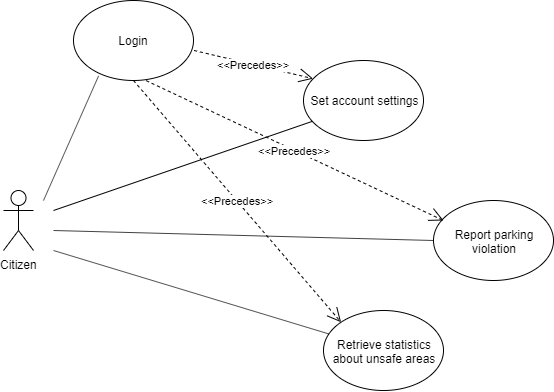
\includegraphics[scale=0.5]{img/use_case_diagrams/citizen.png}
    \caption{\textit{Citizen} Use Case Diagram}
\end{figure}
\clearpage
\begin{figure}[h!]
    \centering
    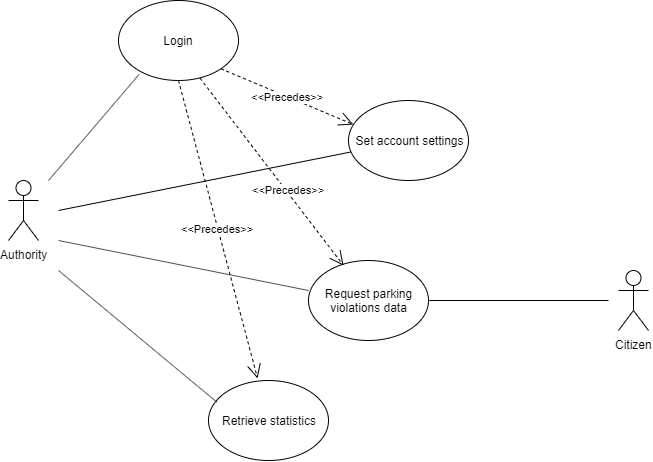
\includegraphics[scale=0.5]{img/use_case_diagrams/authority.png}
    \caption{\textit{Authority} Use Case Diagram}
\end{figure}

\subsubsection{Scenarios}
\begin{itemize}
    \item \textbf{Scenario 1}:
    Luca is walking towards work when outside, in the street of his house, he sees that many cars are parked badly. 
    Some of these are parked near the strips, obstructing the view of the pedestrian who must cross the strips. 
    Luca tired of the situation, that endangers him and many other \textit{Citizens}, decides to report the incident. 
    With his smartphone he opens \textit{SafeStreets} application and after logging in, clicks on the report button to report the fact. 
    He takes the photo by clicking on the report button in the application's home, then he receives the data retrieved, the plate is correctly 
    recognized and, after inserted the type of violation, Luca clicks on confirm button.

    \item \textbf{Scenario 2}:
    Andrea is a disabled boy, he is perfectly able to drive the car but it is difficult for him to walk for long distances. 
    The area in which he works is very busy and it is very rare to find parking nearby, fortunately there are parking 
    spaces reserved for disabled people near the entrance of the building. One morning he finds the place occupied and looking 
    better the machine parked he notice that lack of the certificate necessary for parking in the places reserved for the disabled. 
    Thanks to \textit{SafeStreets} after logging in as a \textit{Citizen}, Andrea can report this violation directly to the \textit{Authorities}. 
    Andrea can now take a photo directly from the application's home by clicking on report button. \textit{SafeStreets} retrieves information such as 
    location and a timestamp with date and time. The application tries to recognize the license plate from the photos and shows the results to Andrea, 
    who after confirming the correctness can click on confirm button and officially send the violation.

    \item \textbf{Scenario 3}:
    The command of the municipal of the municipality of Milan wants to optimize his patrols, aiming at the most problematic areas of the city.
    This targeted surveillance is essential and would bring significant benefits including: a potential reduction of violations in these areas
    and reduction of unnecessary patrols in areas with fewer violations. Fortunately, having joined the \textit{SafeStreets} initiative, thanks to the 
    contribution of \textit{Citizens}, they can use the application to receive these statistics directly from smartphones. After having 
    registered as an \textit{Authority} and logged in, they can access the violations statistics. From this page they can see not only a map with a general
    perspective of the areas but also check for a specific location by moving the pointer on the map.  

    \item \textbf{Scenario 4}:
    Maurizio is a young policeman from the city of Milan. He loves putting a lot of passion into his work and to do so he often learns about new 
    technologies. After downloading \textit{SafeStreets} and registering as an \textit{Authority}, he immediately takes an interest in the function to generate traffic tickets 
    thanks to the reports made by \textit{Users}. From the home of \textit{SafeStreets} Maurizio clicks on retrieve violations button, then the application 
    starts showing to him some violations, once a time with a photo and the related data. Maurizio then needs only to analyze the photo and
    check if it's a valid violations or not. Once he decided he can generate a ticket for that violation and then confirming by clicking on yes/no button. 
    Every answer provided allow \textit{SafeStreets} to update statistics and give more precise information to \textit{Users}. 
\end{itemize}

\subsubsection{Use Cases}
\clearpage
\begin{table}
    \begin{center}
    \centering
\begin{tabular}{ | l | l |}
\hline
\textbf{ID} & UC1 \\
\hline
\textbf{Description} & A \textit{Guest} creates a \textit{Citizen} account \\
\hline
\textbf{Actors} & \textit{Guest} \\
\hline
\textbf{Precondition} & \textit{Guest}'s smartphone satisfies hardware limitations \\
             & \textit{Guest} has downloaded the app from the store \\
             & \textit{Guest} has not an account\\ 
\hline
\textbf{Flow of events} & 1. \textit{Guest} opens the app \\
                        & 2. \textit{Guest} clicks the registration button \\
                        & 3. \textit{System} shows the \textit{Citizen} registration form \\
                        & 4. \textit{Guest} fills the form with his personal data plus mail and password \\
                        & 5. \textit{System} checks the validity of the data inserted \\
                        & 6. \textit{System} sends confirmation email \\
                        & 7. \textit{Guest} receives the email and clicks the URL to complete the registration \\  
\hline
\textbf{Postconditions} & \textit{System} has stored a new \textit{Citizen} account  \\
                        & \textit{Guest} can login as \textit{Citizen} \\
\hline
\textbf{Exceptions} & \textit{Guest} inserts an email that has been used by another account \\
                    & \textit{Guest} inserts a FC that has been inserted by another account \\
                    & \textit{Guest} inserts an invalid FC \\
                    & In these case \textit{System} shows \textit{User} an error message and the flow of events  \\
                    & restart from point 3 \\  
\hline
\end{tabular}
\caption{\textit{Guest} creates a \textit{Citizen} account}
\end{center}
\end{table}


\clearpage
\begin{table}
    \begin{center}
    \centering
\begin{tabular}{ | l | l |}
\hline
\textbf{ID} & UC2 \\
\hline
\textbf{Description} & A \textit{Guest} creates an \textit{Authority} account \\
\hline
\textbf{Actors} & \textit{Guest} \\
\hline
\textbf{Precondition} & \textit{Authority}'s smartphone satisfies hardware limitations \\
             & \textit{Guest} has downloaded the app from the store \\
             & \textit{Guest} has not an account\\ 
\hline
\textbf{Flow of events} & 1. \textit{Guest} opens the app \\
                        & 2. \textit{Guest} clicks the registration button \\
                        & 3. \textit{System} shows the \textit{Citizen} registration form \\
                        & 4. \textit{Guest} clicks on register for \textit{Authority} button \\
                        & 5. \textit{System} shows the \textit{Authority} registration form \\
                        & 6. \textit{Guest} fills the form with his personal data plus Matricola, mail and password \\
                        & 7. \textit{System} checks the validity of the data inserted \\
                        & 8. \textit{System} sends confirmation email \\
                        & 9. \textit{Guest} receives the email and clicks the URL to complete the registration \\  
\hline
\textbf{Postconditions} & \textit{System} has stored a new \textit{Authority} account  \\
                        & \textit{Guest} can login as \textit{Authority} \\
\hline
\textbf{Exceptions} & \textit{Guest} inserts an email that has been used by another account \\
                    & \textit{Guest} inserts a Matricola that has been inserted by another account \\
                    & \textit{Guest} inserts an invalid Matricola \\
                    & In these case \textit{System} shows \textit{User} an error message and the flow of events  \\
                    & restart from point 5 \\  
\hline
\end{tabular}
\caption{\textit{Guest} creates an \textit{Authority} account}
\end{center}
\end{table}

\clearpage
\begin{table}
    \begin{center}
    \centering
\begin{tabular}{ | l | l |}
\hline
\textbf{ID} & UC3 \\
\hline
\textbf{Description} & A \textit{User} logs in  \\
\hline
\textbf{Actors} & \textit{Citizen}, \textit{Authority}\\
\hline
\textbf{Precondition} & \textit{User} has already created the account \\
\hline
\textbf{Flow of events} & 1. \textit{User} opens the app \\
                        & 2. \textit{System} shows login/register interface \\
                        & 3. \textit{User} inputs his credentials \\
                        & 4. \textit{User} clicks login button  \\
                        & 5. \textit{System} checks the validity of the data inserted \\
\hline
\textbf{Postconditions} & \textit{User} can use properly the app   \\
\hline
\textbf{Exceptions} & \textit{User} inserts wrong credentials \\
                    & In this case \textit{System} shows \textit{User} an error message and the flow of events  \\
                    & restart from point 2\\  
\hline
\end{tabular}
\caption{\textit{User} login}
\end{center}
\end{table}

\clearpage

\begin{table}
    \begin{center}
    \centering
\begin{tabular}{ | l | l |}
\hline
\textbf{ID} & UC4 \\
\hline
\textbf{Description} & A \textit{Citizen} reports a parking violation  \\
\hline
\textbf{Actors} & \textit{Citizen} \\
\hline
\textbf{Precondition} & \textit{Citizen} has already logged in \\
\hline
\textbf{Flow of events} & 1. \textit{System} opens the photocamera \\
                        & 2. \textit{Citizen} clicks the report button \\
                        & 3. \textit{System} shows the report info page for \textit{Citizens} \\
                        & 4. \textit{Citizen} inputs the type of violation \\
                        & 5. \textit{Citizen} checks the correctness of the license plate \\
                        & 6. \textit{Citizen} clicks the send button \\
\hline
\textbf{Postconditions} & \textit{System}'s DB stores the violation  \\
\hline
\textbf{Exceptions} & \textit{Citizen} takes a bad picture \\
                    & In this case \textit{System} discards the picture and the flow of events  \\
                    & restart from point 1\\  
\hline
\end{tabular}
\caption{\textit{Citizen} reports a parking violation}
\end{center}
\end{table}

\clearpage
\begin{table}
    \begin{center}
    \centering
\begin{tabular}{ | l | l |}
\hline
\textbf{ID} & UC5 \\
\hline
\textbf{Description} & An \textit{Authority} retrieves a legitimate parking violation  \\
\hline
\textbf{Actors} & \textit{Authority} \\
\hline
\textbf{Precondition} & \textit{Authority} has already logged in \\
\hline
\textbf{Flow of events} & 1. \textit{Authority} clicks the retrieve button \\
                        & 2. \textit{System} shows the report info page for \textit{Authorities} \\
                        & 3. \textit{Authority} checks that it is a real parking violations  \\
                        & 4. \textit{Authority} clicks the YES button  \\
\hline
\textbf{Postconditions} &  \textit{Authority} generates a traffic ticket and \textit{System} uploads \\ 
                        & statistics \\
\hline
\textbf{Exceptions} & \\ 
\hline
\end{tabular}
\caption{Legitimate parking violation retrieved by \textit{Authority} }
\end{center}
\end{table}

\clearpage
\begin{table}
    \begin{center}
    \centering
\begin{tabular}{ | l | l |}
\hline
\textbf{ID} & UC6 \\
\hline
\textbf{Description} & A \textit{Authority} retrieves a wrong parking violation  \\
\hline
\textbf{Actors} & \textit{Authority} \\
\hline
\textbf{Precondition} & \textit{Authority} has already logged in \\
\hline
\textbf{Flow of events} & 1. \textit{Authority} clicks the retrieve button \\
                        & 2. \textit{System} shows the report info page for \textit{Authorities} \\
                        & 3. \textit{Authority} checks that it is not a real parking violations \\
                        & 4. \textit{Authority} clicks the NO button  \\
\hline
\textbf{Postconditions} & \textit{Authority} discards the picture and \textit{System} uploads   \\
                        &  statistics \\
\hline
\textbf{Exceptions} & \\ 
\hline
\end{tabular}
\caption{Wrong parking violation retrieved by \textit{Authority} }
\end{center}
\end{table}

\clearpage
\begin{table}
    \begin{center}
    \centering
\begin{tabular}{ | l | l |}
\hline
\textbf{ID} & UC7 \\
\hline
\textbf{Description} & A \textit{User} retrieves statistics  \\
\hline
\textbf{Actors} & \textit{Authority}, \textit{Citizen} \\
\hline
\textbf{Precondition} & \textit{User} has already logged in \\
\hline
\textbf{Flow of events} & 1. \textit{User} clicks the retrieve statistics button \\
                        & 2. \textit{System} shows summary of statistics \\
\hline
\textbf{Postconditions} & \textit{User} increases his knowledge about parking violations of his city  \\
\hline
\textbf{Exceptions} & \\ 
\hline
\end{tabular}
\caption{statistics retrieved by \textit{User} }
\end{center}
\end{table}

\clearpage

\subsubsection{Sequence Diagrams}
\paragraph{Login}
The following diagram shows how a generic \textit{User} can login into the application. The actors involved
are both \textit{Citizen} and \textit{Authority}.  
\begin{figure}[H]
    \centering
    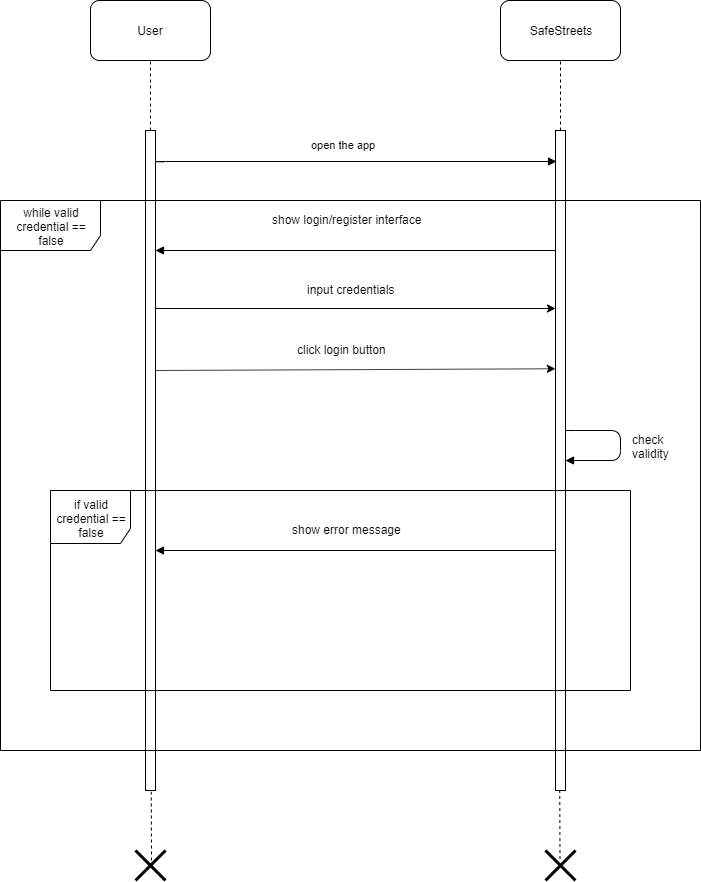
\includegraphics[scale=0.5]{img/sequence_diagrams/login.png}
    \caption{Login}
\end{figure}

\clearpage 

\paragraph{Register Citizen}
This sequence diagram shows how registration process occur in \textit{Citizen} case, the first steps are mandatory to reach
the register page, then until the \textit{User} inserts valid credentials the \textit{System} don't allow him to go next.  
\begin{figure}[H]
    \centering
    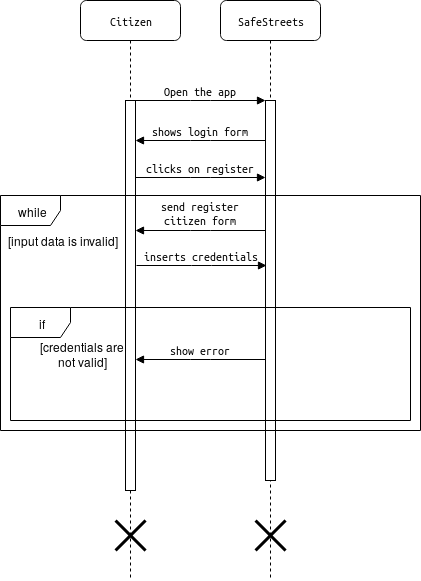
\includegraphics[scale=0.5]{img/sequence_diagrams/register_citizen.png}
    \caption{Register for \textit{Citizen}}
\end{figure}

\clearpage

\paragraph{Register Authority}
Thi sequence diagram represents the same case as above but referred to \textit{Authorities}, so is necessary another
step in order to reach the regster form. Then like in the previous case it's possible to complete correctly the registration
only by inserting valid credentials.

\begin{figure}[H]
    \centering
    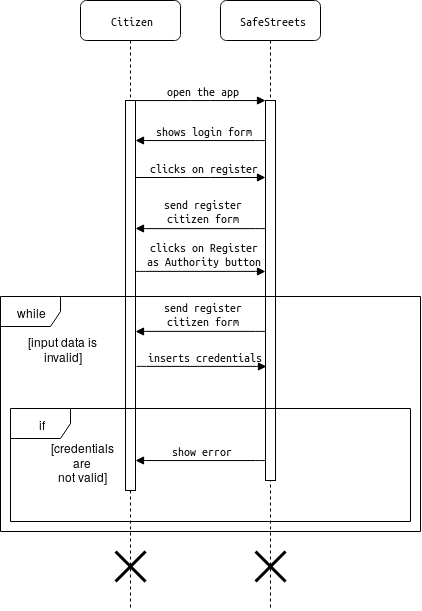
\includegraphics[scale=0.5]{img/sequence_diagrams/register_authority.png}
    \caption{Register for \textit{Authority}}
\end{figure}

\clearpage

\paragraph{Retrieve Violation}
The following diagram shows how an \textit{Authority} can retrieve violations. Two cases are considered: in the 
first case the violation is legitimate, he accepts it and generates traffic ticket. In the second case the violation
is wrong so he discards it. 
\begin{figure}[H]
    \centering
    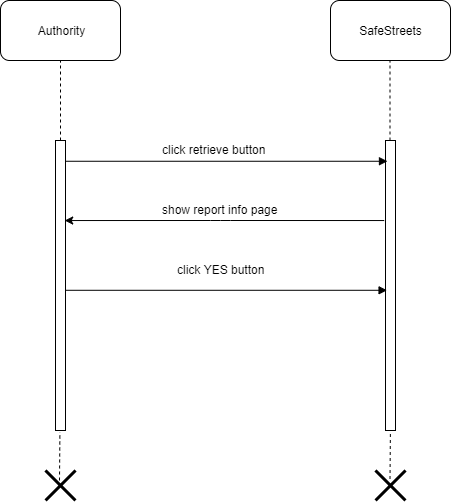
\includegraphics[scale=0.4]{img/sequence_diagrams/accept_retrieve_violation.png}
    \caption{Accept retrieve violation}
\end{figure}

\begin{figure}[H]
    \centering
    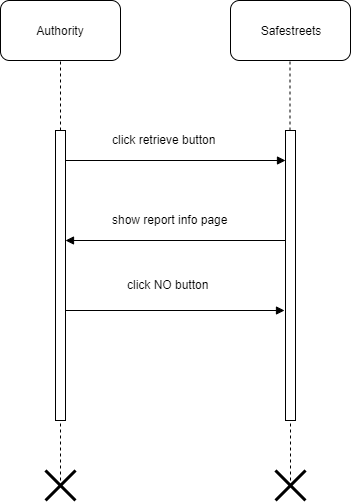
\includegraphics[scale=0.4]{img/sequence_diagrams/discard_retrieve_violation.png}
    \caption{Discard retrieve violation}
\end{figure}

\clearpage

\paragraph{Report violation}
The following diagram shows how a \textit{Citizen} can report a violation. After clicking on report the 
\textit{System} receives data, checks the correctness and tries to recognize the license plate. After \textit{Citizen} 
confirmation the report is officially sended. 

\begin{figure}[H]
    \centering
    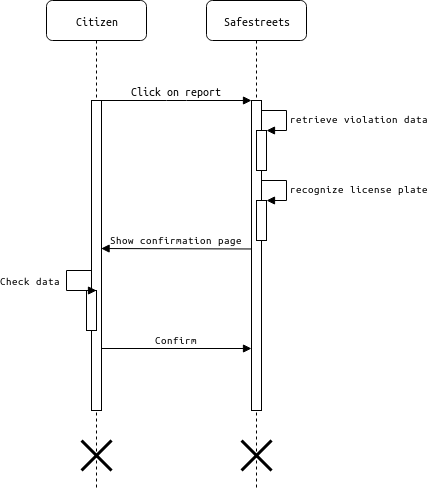
\includegraphics[scale=0.5]{img/sequence_diagrams/report_violation.png}
    \caption{Report violation}
\end{figure}

\clearpage

\paragraph{Retrieve statistics}
The following diagram shows how a generic \textit{User} can retrieve statistics. The actors involved
are both \textit{Citizen} and \textit{Authority}.  
\begin{figure}[H]
    \centering
    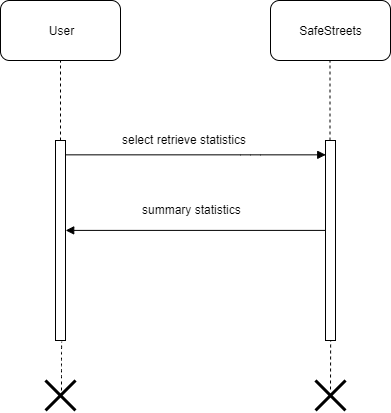
\includegraphics[scale=0.5]{img/sequence_diagrams/retrieve_statistics.png}
    \caption{Retrieve statistics}
\end{figure}


\subsubsection{Goal Mapping on Requirements}
For each goal now will be described below the requirements:
\begin{itemize}
    \item \textbf{[G1]}: Allow \textit{Guests} to be registered as a \textit{Citizen} or as \textit{Authority};
    \begin{itemize}
        \item \textbf{[R1]}: Account can be created if and only if \textit{User} provides unique email and password.
        \item \textbf{[R2]}: The \textit{System} allow \textit{Guest} to create \textit{Citizen} or \textit{Authority} account.
        \item \textbf{[D1]}: \textit{Users} can't make more than one account.
        \item \textbf{[D2]}: The personal informations provided by \textit{User} are valid and belongs to him. 
    \end{itemize}

    \item \textbf{[G2]}: Allow \textit{Citizens} to report parking violations;
    \begin{itemize}
        \item \textbf{[R3]}: The \textit{Citizen} has to take the violation's photo with the application. 
        \item \textbf{[R4]}: The \textit{System} allows \textit{Citizen} to input some violation's data.
        \item \textbf{[R5]}: The photo taken must be recognizable by the \textit{System}.  
        \item \textbf{[R6]}: The \textit{Citizen} has to be able to discard the photo taken.
        \item \textbf{[R7]}: The \textit{System} has to be able to attach the correct date, time and position to the report.
        \item \textbf{[R8]}: The \textit{Citizen} can't change date, time and position in the report.
        \item \textbf{[D3]}: Position data has an accuracy of 10 meters.
        \item \textbf{[D4]}: The \textit{System} can access internet whenewer needs it.
        \item \textbf{[D5]}: Permission to access GPS data is always allowed.
        \item \textbf{[D6]}: Permission to take a photo is always allowed. 
    \end{itemize}

    \item \textbf{[G3]}: \textit{Citizen} has to be able to input information about the violation that he has reported;
    \begin{itemize}
        \item \textbf{[R9]}: \textit{Citizen} can change the license plate if it isn't recognised properly.
        \item \textbf{[R10]}: \textit{Citizen} has to be able to choose the correct type of violation.
    \end{itemize}

    \item \textbf{[G4]}: Must provide a visualization of the areas with high frequency of violations to \textit{Users};
    \begin{itemize}
        \item \textbf{[R11]}: \textit{Users} can change the area of visualization.
        \item \textbf{[R12]}: \textit{Users} can change the date of visualization. 
        \item \textbf{[D3]}: Position data as an accuracy of 10 meters.
        \item \textbf{[D4]}: The \textit{System} can access internet whenewer needs it.
        \item \textbf{[D5]}: Permission to access GPS data is always allowed.
    \end{itemize}

    \item \textbf{[G5]}: Must provide a visualization of vehicles that commit the most violations to \textit{Authorities}; 
    \begin{itemize}
        \item \textbf{[R13]}: \textit{Authority} can search for a specific license plate.
        \item \textbf{[R14]}: \textit{Users} can change the date of visualization.
        \item \textbf{[D4]}: The \textit{System} can access internet whenewer needs it.
        \item \textbf{[D5]}: Permission to access GPS data is always allowed.
    \end{itemize}

    \item \textbf{[G6]}: Must ensure the chain of custody of the information sent by \textit{Citizens};
    \begin{itemize}
        \item \textbf{[R15]}: Violations sent must be digitally signed and hashed.
        \item \textbf{[R16]}: The \textit{System} must use HTTPS to safely communicate.
        \item \textbf{[D4]}: The \textit{System} can access internet whenewer needs it.
    \end{itemize}

    \item \textbf{[G7]}: \textit{Authorities} can retrieve traffic violations in order to generate traffic tickets;
    \begin{itemize}
        \item \textbf{[R17]}: The violation retrieved can only be seen by the \textit{Authority} that retrieves it.
        \item \textbf{[D4]}: The \textit{System} can access internet whenewer needs it.
    \end{itemize}

    \item \textbf{[G8]}: \textit{System} must build statistics with the informations about issued tickets;
    \begin{itemize}
        \item \textbf{[R18]}: The \textit{System} must update the statistics with the most recent data.
    \end{itemize}
\end{itemize}

\subsection{Performance Requirements}
In this section we discuss requirements for what regards performance. The \textit{System} must be able to support up to
5 million of registered \textit{Users}. This limitation is not posed by the front-end of the \textit{System}, but rather by the 
back-end part, specifically the DB. For the same reasons it must be able to handle up to 10 million of parking violations 
sent by the \textit{Citizen}. In order to avoid any kind of saturation, every parking violation that has not been taken into account
by any \textit{Authority} for 30 days, must be automatically discarded. This operation does not update the information about 
statistics.
 \\Requests about statistics shall be processed in less than 5 seconds. Requests about parking violations, instead, shall be processed 
 in less than 1 second.     

\subsection{Design Constraints}
\subsubsection{Standards compliance}
The S2B  will use certain measures as:
\begin{itemize}
    \item Standard longitude and latitude measures for the position.
\end{itemize}
For what concerns the privacy, the S2B is subject to GDPR, a regulation in EU law on data protection 
and privacy for all individual \textit{Citizens} of UE.  

\subsubsection{Hardware limitations}
In order to work properly the application must rely on hardwares that have certain requirements 
such as:
\begin{itemize}
    \item GPS
    \item internet connection (4G/3G/2G)
    \item Photocamera with a minimum precision of 5Mp 
\end{itemize}   

\subsection{Software System Attributes}

\subsubsection{Reliability}
The \textit{System} must be able to run continuously without any interruptions. In order to do that, it must be ensured 
that the \textit{System} is fault tolerant. To prevent downtime, one of the main goals of architecture design must be 
ensuring graceful degradation of the \textit{System}.

\subsubsection{Availability}
\textit{SafeStreets} does not present any critical functions so 99\% availability with 3.65 days/year
as downtime should be good.  

\subsubsection{Security}
Security is a key aspect of \textit{SafeStreets} because it is very important that the informations are never altered.
The S2B must:
\begin{enumerate}
 \item use HTTPS to safely communicate with the Server and DBMS.    
 \item Hash the passwords so that they are not stored in clear in the DB.
 \item Encrypt sensitive data before storing it.
 \item digital sign the parking violations sent by \textit{Citizens} and then hash them.  
\end{enumerate} 

\subsubsection{Maintainability}
In order to achieve maintainability some good practices must be followed to reduce coupling and avoid code duplication.
Modularity is also necessary in order to make the code more robust and to make easier adding new functionalities.

\subsubsection{Portability}
S2B, as it stated previously, will work both in Andorid and iOS and this ensures itself portability. For 
the back-end part, it should be OS independent.

\clearpage

%%%%%%%%%% !CHAPTER 3 %%%%%%%%%%

\section{Formal Analysis with Alloy}

\subsection{A description of The Alloy Model}
In this section we will focus on the relevant part of the application described
using alloy model language. We decided to
focus the model on the interaction between three main objects of 
\textit{SafeStreets} that are: \textit{Citizen}, \textit{Authority} and Reports. 
Those interactions are foundamental in order to reach the application's goals. 
The model will presents an analysis of the main functions such as:
\begin{itemize}
    \item A \textit{Citizen} sends a report. 
    \item An \textit{Authority} confirms a report. 
    \item An \textit{Authority} discards a report.
\end{itemize}
Those functions are expressed by using different predicates. In 
the description of the model we made some semplification in order to
make the model cleaner and more readable. First we have reduced the range
of the position's attributes (i.e. latitude and longitude) by scaling them and 
some non-relevant attributes of objects are omited. 

\clearpage

\subsection{Alloy Model}
\lstinputlisting[language=alloy]{safestreets.als}

\clearpage

\subsubsection{Model Results Images}
\begin{figure}[H]
    \centering
    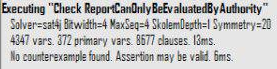
\includegraphics[scale=0.9]{img/alloy/check1.png}
    \caption{Check Report Can Only Be Evaluated By Authority} 
\end{figure}

\begin{figure}[H]
    \centering
    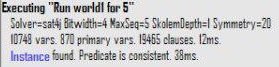
\includegraphics[scale=0.9]{img/alloy/world1.png}
    \caption{World 1}
\end{figure}

\begin{figure}[H]
    \centering
    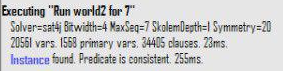
\includegraphics[scale=0.9]{img/alloy/world2.png}
    \caption{World 2}
\end{figure}

\begin{figure}[H]
    \centering
    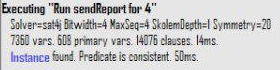
\includegraphics[scale=0.9]{img/alloy/sendReport.png}
    \caption{Send Report}
\end{figure}

\begin{figure}[H]
    \centering
    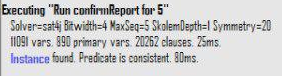
\includegraphics[scale=0.9]{img/alloy/confirmReport.png}
    \caption{Confirm Report}
\end{figure}

\begin{figure}[H]
    \centering
    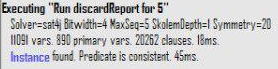
\includegraphics[scale=0.9]{img/alloy/discardReport.png}
    \caption{Discard Report}
\end{figure}

\clearpage

\subsubsection{Model Graphical Images}

\begin{figure}[H]
    \centering
    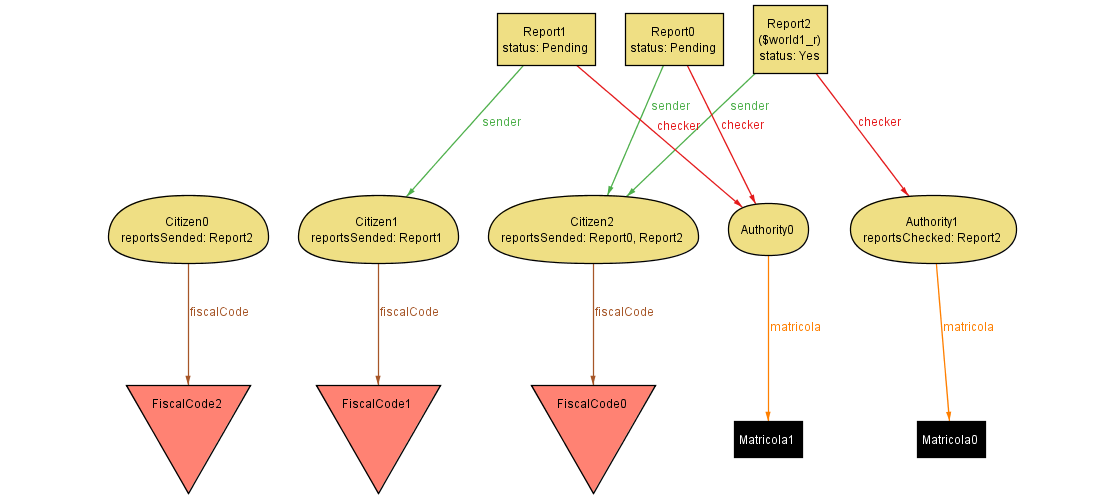
\includegraphics[scale=0.4]{img/alloy/world1_magic.png}
    \caption{World 1}
\end{figure}

\begin{figure}[H]
    \centering
    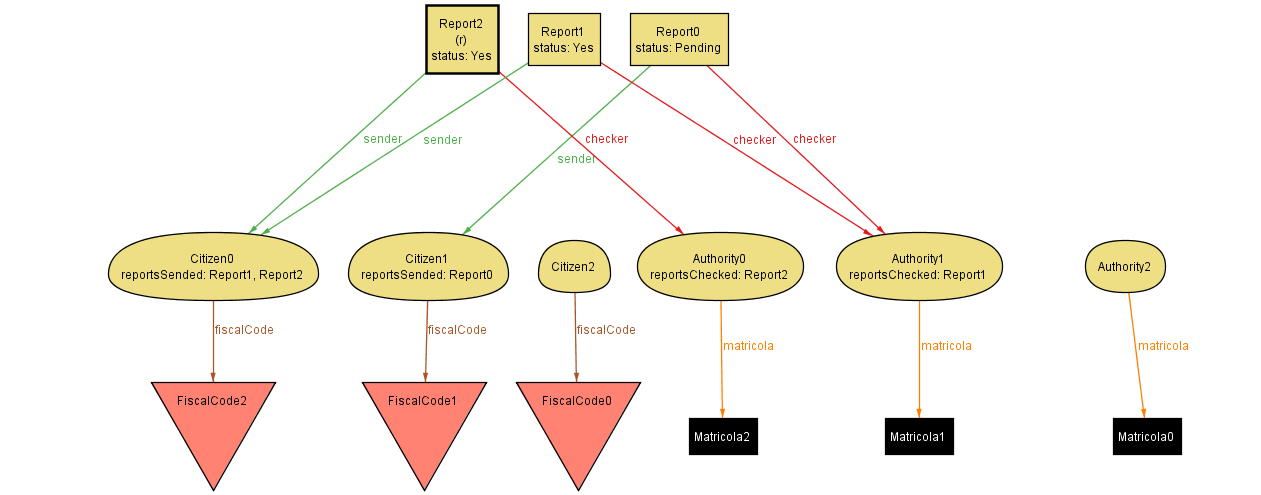
\includegraphics[scale=0.4]{img/alloy/world2_magic.png}
    \caption{World 2}
\end{figure}

\begin{figure}[H]
    \centering
    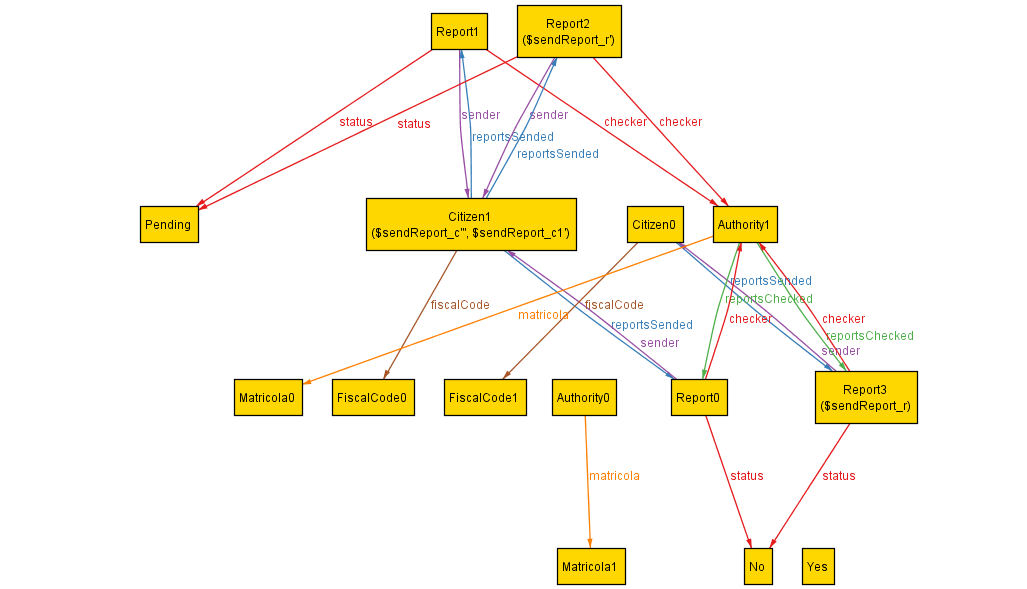
\includegraphics[scale=0.4]{img/alloy/graphical_sendReport.png}
    \caption{Send Report}
\end{figure}

\begin{figure}[H]
    \centering
    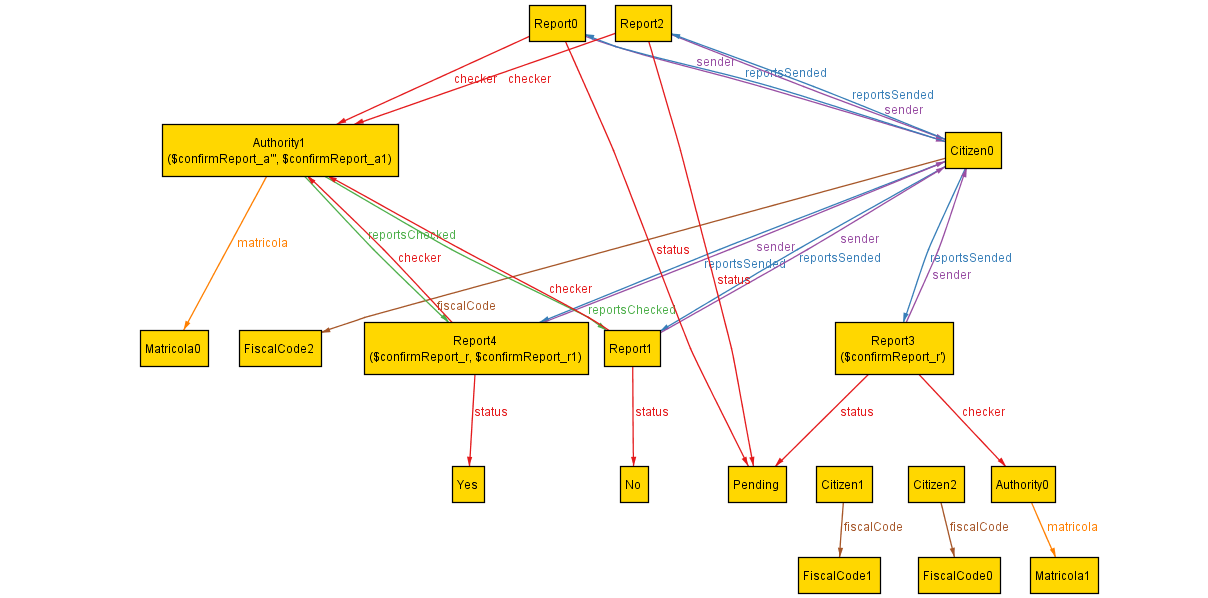
\includegraphics[scale=0.4]{img/alloy/graphical_confirmReport.png}
    \caption{Confirm Report}
\end{figure}

\begin{figure}[H]
    \centering
    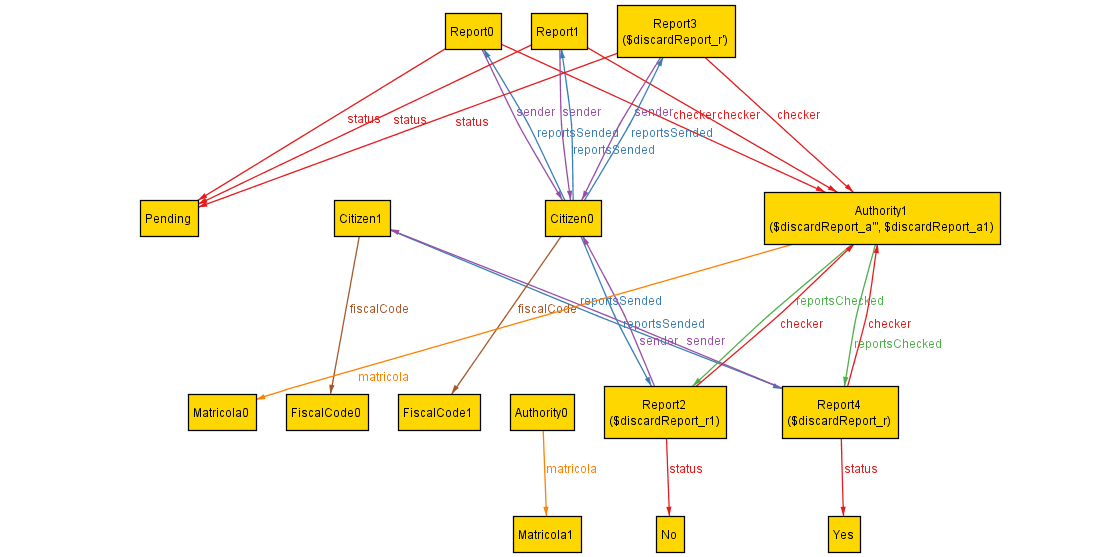
\includegraphics[scale=0.4]{img/alloy/graphical_discardReport.png}
    \caption{Discard Report}
\end{figure}

\section{Efforts}
\begin{center}
    \begin{tabular}{ | l | l | l |}
        \hline
        Efforts & Dario & Pierriccardo \\
        \hline
        initial setup latex and github & 3h & 3h \\
        \hline
        chapter 1 & 6h & 6h \\
        \hline
        chapter 2 & 7h & 7h \\
        \hline
        chapter 3 & 10h & 10h \\
        \hline
        chapter 4 & 15h & 15h \\
        \hline
        total & 41h & 41h \\
        \hline
    \end{tabular}
    \end{center}
\end{document}